%\documentclass[
  bibliography=totoc,     % Literatur im Inhaltsverzeichnis
  captions=tableheading,  % Tabellenüberschriften
  titlepage=firstiscover, % Titelseite ist Deckblatt
]{scrartcl}

% Paket float verbessern
\usepackage{scrhack}

% Warnung, falls nochmal kompiliert werden muss
\usepackage[aux]{rerunfilecheck}

% unverzichtbare Mathe-Befehle
\usepackage{amsmath}
% viele Mathe-Symbole
\usepackage{amssymb}
% Erweiterungen für amsmath
\usepackage{mathtools}

% Fonteinstellungen
\usepackage{fontspec}
% Latin Modern Fonts werden automatisch geladen
% Alternativ zum Beispiel:
%\setromanfont{Libertinus Serif}
%\setsansfont{Libertinus Sans}
%\setmonofont{Libertinus Mono}

% Wenn man andere Schriftarten gesetzt hat,
% sollte man das Seiten-Layout neu berechnen lassen
\recalctypearea{}

% deutsche Spracheinstellungen
\usepackage[ngerman]{babel}


\usepackage[
  math-style=ISO,    % ┐
  bold-style=ISO,    % │
  sans-style=italic, % │ ISO-Standard folgen
  nabla=upright,     % │
  partial=upright,   % │
  mathrm=sym,        % ┘
  warnings-off={           % ┐
    mathtools-colon,       % │ unnötige Warnungen ausschalten
    mathtools-overbracket, % │
  },                       % ┘
]{unicode-math}

% traditionelle Fonts für Mathematik
\setmathfont{Latin Modern Math}
% Alternativ zum Beispiel:
%\setmathfont{Libertinus Math}

\setmathfont{XITS Math}[range={scr, bfscr}]
\setmathfont{XITS Math}[range={cal, bfcal}, StylisticSet=1]

% Zahlen und Einheiten
\usepackage[
  locale=DE,                   % deutsche Einstellungen
  separate-uncertainty=true,   % immer Unsicherheit mit \pm
  per-mode=symbol-or-fraction, % / in inline math, fraction in display math
]{siunitx}

% chemische Formeln
\usepackage[
  version=4,
  math-greek=default, % ┐ mit unicode-math zusammenarbeiten
  text-greek=default, % ┘
]{mhchem}

% richtige Anführungszeichen
\usepackage[autostyle]{csquotes}

% schöne Brüche im Text
\usepackage{xfrac}

% Standardplatzierung für Floats einstellen
\usepackage{float}
\floatplacement{figure}{htbp}
\floatplacement{table}{htbp}

% Floats innerhalb einer Section halten
\usepackage[
  section, % Floats innerhalb der Section halten
  below,   % unterhalb der Section aber auf der selben Seite ist ok
]{placeins}

% Seite drehen für breite Tabellen: landscape Umgebung
\usepackage{pdflscape}

% Captions schöner machen.
\usepackage[
  labelfont=bf,        % Tabelle x: Abbildung y: ist jetzt fett
  font=small,          % Schrift etwas kleiner als Dokument
  width=0.9\textwidth, % maximale Breite einer Caption schmaler
]{caption}
% subfigure, subtable, subref
\usepackage{subcaption}

% Grafiken können eingebunden werden
\usepackage{graphicx}

% schöne Tabellen
\usepackage{tabularray}
\UseTblrLibrary{booktabs, siunitx}

% Verbesserungen am Schriftbild
\usepackage{microtype}

% Literaturverzeichnis
\usepackage[
  backend=biber,
]{biblatex}
% Quellendatenbank
\addbibresource{lit.bib}
\addbibresource{programme.bib}

% Hyperlinks im Dokument
\usepackage[
  german,
  unicode,        % Unicode in PDF-Attributen erlauben
  pdfusetitle,    % Titel, Autoren und Datum als PDF-Attribute
  pdfcreator={},  % ┐ PDF-Attribute säubern
  pdfproducer={}, % ┘
]{hyperref}
% erweiterte Bookmarks im PDF
\usepackage{bookmark}

% Trennung von Wörtern mit Strichen
\usepackage[shortcuts]{extdash}

\author{%
  Vincent Wirsdörfer\\%
  \href{mailto:vincent.wirsdoerfer@udo.edu}{authorA@udo.edu}%
  \and%
  Joris Daus\\%
  \href{mailto:joris.daus@udo.edu}{authorB@udo.edu}%
}
\publishers{TU Dortmund – Fakultät Physik}


%\begin{document}

\section{Versuchsaufbau}
\label{sec:Versuchsaufbau}

Grundlage des Experiments ist eine Hochdruck-Quecksilberdampflampe (Hg Lampe), welche polychromatisches Licht emittiert. Dieses Licht fällt auf eine
Sammellinse mit einer Brennweite von $f = \qty{50}{\milli\meter}$. Durch die Linse kann das Licht der Hg Lampe auf den darauf folgenden Spalt abgebildet 
werden. Über eine weitere Linse wird das Licht kollimiert, sprich in Parallelrichtung weitergeleitet und trifft resultierend auf ein Geradsichtprisma, 
welches das Licht spektral zerlegt. Das ursprünglich polychromatische Licht ist somit in Spektrallinien verschiedener Wellenlängen und Frequenzen 
diskretisiert. Dieses monochromatische Licht strahlt folglich auf eine Vakuum-Photozelle, welche die in der Theorie \ref{sec:Theorie} benannten 
Phänomene zum Vorschein bringen soll. Hauptbestandteil der Photozelle ist ein evakuierter Glaskolben, welcher von innen mit einer Metallschicht bedampft
ist und die Kathode des Versuchs repräsentiert. Über einen Schwenkarm kann die Photozelle ausgerichtet werden, sodass die einzelnen Spektralfarben auf die 
Metallkathode einfallen können. Zusätzlich verfügt die Photozelle über einen Anodenring aus einer Platin-Rhodium Legierung. Die Anlegung
einer Spannung zwischen Kathode und Anode kann je nach Ausrichtung des elektrischen Feldes die herausgelösten Elektronen beschleunigen oder abbremsen. 
Über ein Picoamperemeter kann der Photostrom gemessen werden. Die Anordnung der soeben beschriebenen Elemente entspricht der folgenden Ansicht.\\

\begin{figure}
    \centering
    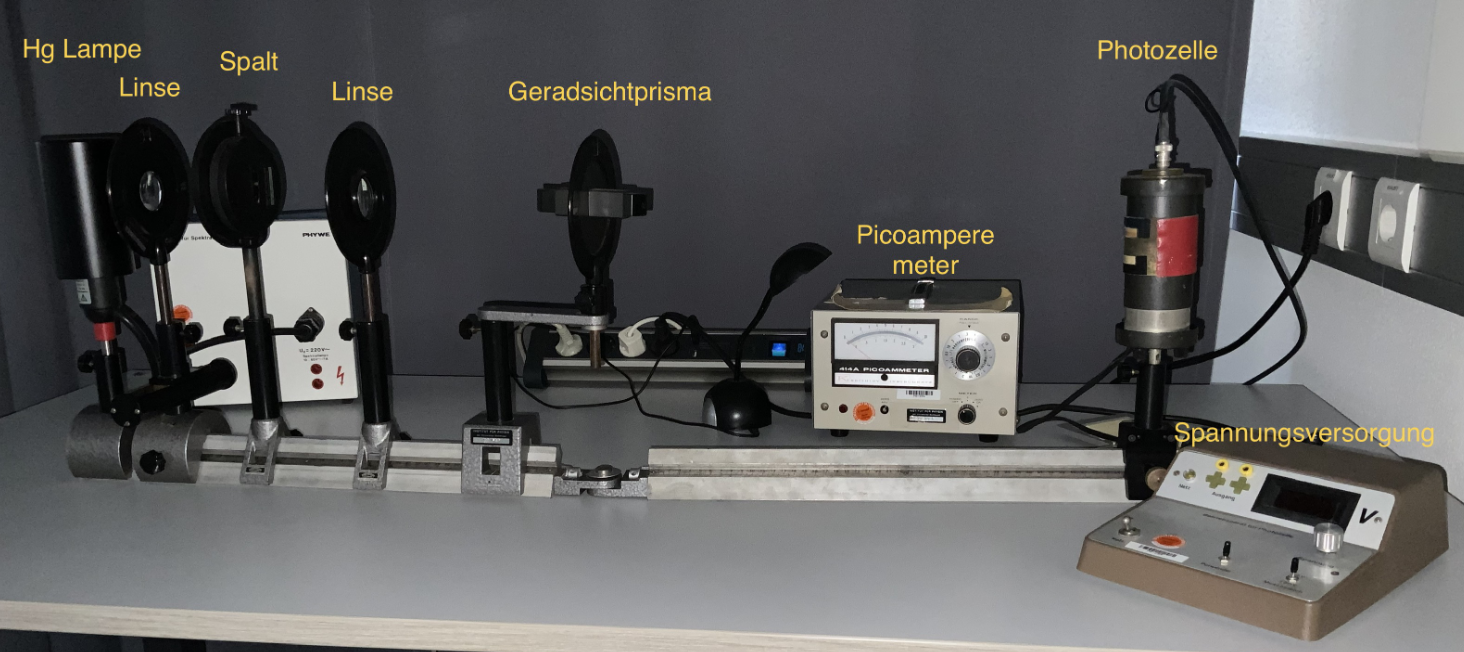
\includegraphics[height=5cm]{content/Anordnung.png}
    \caption{Anordnung der Versuchselemente zum Photoeffekt\cite{Versuchsanleitung_v500}.}
    \label{fig:Anordnung}
\end{figure}


\section{Versuchsdurchführung}
\label{sec:Versuchsdurchfuehrung}

Zu Beginn des Versuchs wird die korrekte Positionierung aller Bestandteile des Experiments überprüft und ggf. korrigiert. Nach Einschalten der Quecksilberdampflampe
kann die Schärfe der Linienspektren über Variation der Abstände zwischen Linse, Spalt und Prisma kontrolliert werden. Mittels des Schwenkarms kann somit 
die blaue Linie des Lichtspektrums auf die Kathode der Photozelle einfallen. Nach Aktivierung der Spannungsversorgung und des Picoamperemeters wird ein 
Photostrom durch die emittierten Elektronen gemessen. 

\subsection{Aufnahme der Strom-Spannungskennlinien}

Im ersten Versuchsteil wird eine präzise Messung der Strom-Spannungskennlinie der blauen Spektrallinie durchgeführt. Hierfür wird zunächst die Intensität des 
Lichts maximiert, indem die Spaltbreite über einen Regler vergrößert wird. Ist dies geschehen, so wird jene Spannung eingestellt, welche den Photostrom verschwinden
lässt. Diese Spannung wird als \emph{Grenzspannung} $U_\text{g}$ bezeichnet. Im Folgenden werden kleine Intervallschritte um die Grenzspannung gesammelt und 
die zugehörigen Stromstärken notiert. Ab einem gewissen Spannungswert werden die Intervallschritte sukzessive erhöht, bis der Sättigungsstrom erreicht ist\footnote{
Aufgrund der Tatsache, dass die Messwerte der Gruppen vertauscht wurden, kann die explizite Veränderung der Schrittgröße nur erschwert wiedergegeben werden.}. 
Neben den Tupeln an Spannungs- und Stromwerten wird auch der Sättigungsstrom aufgenommen.\\

%\subsection{Großschrittige Messung bei mittlerer Lichtintensität}

\noindent Anschließend wird eine ähnliche Messung bei halber Intensität durchgeführt. Dazu wird die Spaltbreite erneut so angepasst, dass sich die einzelnen Spektralfarben
gerade nicht überdecken. Kontrolliert wird dies mittels einer Teilnehmerkarte, welche als Schirm des spektral zerlegten Lichts fungiert. Nach Einstellung 
der Grenzspannung, wird nun die Spannung instant in größen Schritten erhöht, bis in etwa zehn bis zwölf Stromwerte notiert sind. Neben der blauen Spektralfarbe, wird diese 
globale Strom-Spannungskennlinie auch für grünes, gelbes und violettes Licht aufgenommen. Je nach Positionierung der Farbe wird die Photozelle über den 
Schwenkarm entsprechend ausgerichtet und die obigen Messschritte identisch wiederholt. Ist diese Prozedur für hinreichend viele Spektralfarben ausgeführt, 
können die Geräte ausgeschaltet werden. 


\section{Messwerte}

Die präzise und globale Messung der blauen Spektralfarbe ergibt die folgenden Daten der Strom- und Spannungszugehörigkeit.

\begin{table}[H]
    \caption{Präzise Messung bei hoher Lichtintensität.}
    \label{tab:PraeziseBlauGlobal}
    \begin{minipage}[t]{0.5\textwidth}
        \vspace{0pt}
        \centering
    \begin{tblr}{
        colspec = {S[table-format=1.2] S[table-format=1.3]},
        row{1} = {guard, mode = math},
        }
        \toprule
            \text{Spannung} \mathbin{/} \unit{\volt} & \text{Stromstärke} \mathbin{/} \unit{\nano\ampere} \\
        \midrule
        -1.14  &  0     \\
        -1.13  &  0.005 \\
        -1.12  &  0.007 \\
        -1.11  &  0.009 \\
        -1.10  &  0.011 \\
        -1.09  &  0.013 \\
        -1.08  &  0.016 \\
        -1.07  &  0.020 \\
        -1.06  &  0.023 \\
        -1.05  &  0.027 \\
        -1.04  &  0.031 \\
        -1.03  &  0.036 \\
        -1.02  &  0.039 \\
        -1.01  &  0.043 \\
        -1.00  &  0.047 \\
        -0.99  &  0.051 \\
        -0.98  &  0.052 \\
        -0.97  &  0.060 \\
        -0.96  &  0.065 \\
        -0.95  &  0.070 \\
        -0.94  &  0.077 \\
        -0.93  &  0.085 \\
        -0.92  &  0.090 \\
        -0.91  &  0.097 \\
        -0.90  &  0.100 \\
        -0.89  &  0.115 \\
        -0.88  &  0.125 \\
        -0.87  &  0.135 \\
        -0.86  &  0.140 \\
        -0.85  &  0.185 \\
        -0.84  &  0.200 \\
        -0.83  &  0.210 \\
        -0.82  &  0.225 \\
        -0.81  &  0.235 \\
        -0.80  &  0.250 \\
    \end{tblr}
\end{minipage} \hfill
\begin{minipage}[t]{0.5\textwidth}
        \vspace{0pt}
        \centering
    \begin{tblr}{
            colspec={S[table-format=1.2] S[table-format=1.3]},
            row{1} = {guard, mode = math},
        }
        \toprule
            \text{Spannung} \mathbin{/} \unit{\volt} & \text{Stromstärke} \mathbin{/} \unit{\nano\ampere} \\
        \midrule
        -0.79  &  0.265   \\
        -0.78  &  0.275   \\
        -0.77  &  0.300   \\
        -0.70  &  0.400   \\
        -0.60  &  0.660   \\
        -0.50  &  0.960   \\
        -0.40  &  1.30    \\
        -0.30  &  1.90    \\
        -0.20  &  2.30    \\
        -0.10  &  2.60    \\
         0.00  &  3.00    \\ 
         0.10  &  3.20    \\
         0.20  &  3.40    \\
         0.30  &  3.50    \\
         0.40  &  3.70    \\
         0.50  &  4.00    \\
         0.60  &  4.40    \\
         0.70  &  4.60    \\
         0.80  &  4.80    \\
         0.90  &  5.00    \\
         1.00  &  5.40    \\
         2.00  &  7.70    \\
         3.00  &  10.00   \\
         4.00  &  12.00   \\
         5.00  &  13.00   \\
         6.00  &  14.00   \\
         7.00  &  15.00   \\ 
         8.00  &  16.00   \\  
         9.00  &  17.00   \\  
        10.00  &  18.00   \\  
        11.00  &  19.00   \\  
        12.00  &  20.00   \\  
        13.00  &  21.00   \\  
        14.00  &  21.00   \\ 
        15.00  &  21.00   \\ 
        \end{tblr}
    \end{minipage}\hfill
\end{table}

\noindent Die Messwerte der globalen Messung von blau bei halber Intensität werden in der folgenden Tabelle aufgelistet.

\begin{table}[H]
    \centering 
    \caption{Globale Messung der blauen Spektralfarbe bei halber Intensität.}
    \begin{tblr}{
        colspec = {S[table-format=2.0] S[table-format=2.1]},
        row{1} = {guard, mode=math},
        }
        \toprule 
            \text{Spannung} \mathbin{/} \unit{\volt} & \text{Stromstärke} \mathbin{/} \unit{\nano\ampere} \\
        \midrule
        15  &  24.0  \\
        14  &  23.5  \\
        13  &  23.0  \\
        12  &  22.0  \\
        11  &  21.0  \\
        10  &  20.0  \\
        9   &  19.5  \\
        8   &  18.0  \\
        7   &  17.0  \\
        6   &  15.5  \\
        5   &  12.0  \\
        4   &  11.5  \\
        3   &  10.0  \\
        2   &  6.5   \\
        1   &  3.5   \\
        0   &  1.3   \\
        -1  &  0.0   \\
        \bottomrule
    \end{tblr}
    \label{tab:BlauGrobGlobal}
\end{table}

\noindent Die letzten Messreihen beinhalten die Strom- Spannungskennlinien der grünen, gelben und violetten Spektralfarben.

\begin{table}[H]
    %\caption{Tabellen.}
    \label{tab:GruenGelb}
    \begin{minipage}[t]{0.5\textwidth}
        \vspace{0pt}
        \centering
        \caption{Grüne Spektralfarbe.}
    \begin{tblr}{
        colspec = {S[table-format=1.2] S[table-format=1.3]},
        row{1} = {guard, mode = math},
        }
        \toprule
            \text{Spannung} \mathbin{/} \unit{\volt} & \text{Stromstärke} \mathbin{/} \unit{\nano\ampere} \\
        \midrule
        -0.57  &  0     \\
        -0.56  &  0.003 \\
        -0.55  &  0.005 \\
        -0.54  &  0.008 \\
        -0.53  &  0.010 \\
        -0.52  &  0.014 \\
        -0.51  &  0.017 \\
        -0.50  &  0.020 \\
        -0.49  &  0.024 \\
        -0.48  &  0.029 \\
        -0.47  &  0.034 \\
    \end{tblr}
\end{minipage} \hfill
\begin{minipage}[t]{0.5\textwidth}
        \vspace{0pt}
        \centering
        \caption{Gelbe Spektralfarbe.}
    \begin{tblr}{
            colspec={S[table-format=1.2] S[table-format=1.3]},
            row{1} = {guard, mode = math},
        }
        \toprule
            \text{Spannung} \mathbin{/} \unit{\volt} & \text{Stromstärke} \mathbin{/} \unit{\nano\ampere} \\
        \midrule
        -0.45  &  0     \\
        -0.44  &  0.001 \\
        -0.43  &  0.002 \\
        -0.42  &  0.003 \\
        -0.41  &  0.004 \\
        -0.40  &  0.005 \\
        -0.39  &  0.006 \\
        -0.38  &  0.007 \\
        -0.37  &  0.008 \\
        -0.36  &  0.010 \\
        -0.35  &  0.014 \\
        \end{tblr}
    \end{minipage}\hfill
\end{table}

\begin{table}[H]
    \centering 
    \caption{Vioelette Spektralfarbe.}
    \begin{tblr}{
        colspec = {S[table-format=1.2] S[table-format=1.3]},
        row{1} = {guard, mode=math},
        }
        \toprule 
            \text{Spannung} \mathbin{/} \unit{\volt} & \text{Stromstärke} \mathbin{/} \unit{\nano\ampere} \\
        \midrule
        -1.32  &  0     \\
        -1.31  &  0.002 \\
        -1.30  &  0.003 \\
        -1.29  &  0.004 \\
        -1.28  &  0.006 \\
        -1.27  &  0.008 \\
        -1.26  &  0.009 \\
        -1.25  &  0.011 \\
        -1.24  &  0.012 \\
        -1.23  &  0.014 \\
        -1.22  &  0.016 \\
        \bottomrule
    \end{tblr}
    \label{tab:Herzfrequenz}
\end{table}

%\end{document}

